\chapter{Properties of our Analysis}\label{ch:Properties}

In this chapter we discuss some properties of our analysis. First  we
discuss the need of introducing boolean variables on the top of
field sensitive matrices. We then discuss how we guarantee termination of our analysis. 
We also give bounds corresponding to the storage requirement of our analysis.

%%%%%%%%%%%%%%%%%%%%%%%%%%%%%%%%%%%%%%%%%%%%%%%%%%%%%%%%%%%%%%%%%%%%%
\section{Need for Boolean Variables}
%%%%%%%%%%%%%%%%%%%%%%%%%%%%%%%%%%%%%%%%%%%%%%%%%%%%%%%%%%%%%%%%%%%%%

Because we compute approximations for field sensitive
matrices under certain conditions (e.g. for statement $\p =
\q\rightarrow f$), these matrices can result in imprecise
shape. Boolean variables help us retain some precision in
such cases, as demonstrated next.
%
\begin{figure}[t]
  \centering
  \begin{tabular}{@{}lcc@{}}
    \scalebox{0.80}{
      \tt
      \begin{tabular}[b]{l}
        \qquad \qquad \ldots \\
        S1. r = s$\rightarrow$g;\\
        S2. p$\rightarrow$f = q;  \\
        S3. p$\rightarrow$f = NULL; \\
        \qquad \qquad \ldots \\
      \end{tabular}
    } &
    \scalebox{0.8}{\psset{unit=1mm}
    \begin{pspicture} (0,0)(30,16)
      \putnode{p0}{origin}{3}{3}{\pscirclebox[framesep=3pt]{\p}}
      \putnode{s0}{p0}{0}{10}{\pscirclebox[framesep=4pt]{\s}}
      \putnode{t0}{s0}{15}{0}{\pscirclebox[framesep=5pt]{\ }}
      \putnode{q0}{p0}{15}{0}{\pscirclebox[framesep=3pt]{\q}}
      \putnode{u0}{q0}{10}{5}{\pscirclebox[framesep=5pt]{\ }}

      \ncline{->}{s0}{t0}
      \Aput[0.1]{$g$}
      \ncline[nodesep=-0.5]{->}{t0}{p0}
      \Aput[0.1]{$f$}
      \ncline[nodesep=-0.5]{->}{t0}{u0}
      \Aput[0.1]{$g$}
      \ncline[nodesep=-0.5]{->}{q0}{u0}
      \Aput[0.1]{$h$}

    \end{pspicture}}
    &
    \scalebox{0.80}{
    \begin{tabular}[b]{|c|c|c|c|}
      \hline
	  {After} & $f_{pq}$ & $\IFM{r}{q}$                             	    & $\DFM{r}{p}$ \\ \hline
	  {\tt S1}       &  {\tt false}  &  $\upath \times \{h\}$                   & \upath \\ \hline
	  {\tt S2}       &  {\tt true}   &  $\upath \times \{h, \epsilon\}$  & \upath \\ \hline
	  {\tt S3}       &  {\tt false}  &  $\upath \times \{h, \epsilon\}$  & \upath \\ \hline
    \end{tabular}}  \\
    \scalebox{0.80}{(a) A code fragment} &
    \scalebox{0.80}{(b) \begin{tabular}[t]{p{37mm}}
    Heap Structure before {\tt S1} 
    \end{tabular}}
    &     
    \scalebox{0.80}{(c) \begin{tabular}[t]{p{43mm}}
        Values for boolean variable, $D_F$, and
        $I_F$ for relevant pointer fields.
    \end{tabular}}
      \\
  \end{tabular}
  \caption{Using boolean variables to improve
    precision \label{fig:conclusion}} 
\end{figure}

\begin{example} {\rm
 Fig.~\ref{fig:conclusion}(a) shows a program fragment, and
 Fig.~\ref{fig:conclusion}(b) shows a possible heap graph at
 a program point before statement {\tt S1}.  At {\tt S2}, a
 DAG is created that is reachable from \myr\ which gets
 destroyed after {\tt S3}.  
 Fig.~\ref{fig:conclusion}(c) shows the Direction
 ($D_F$) and Interference ($I_F$) matrices at
 various program points.  After statement {\tt S2} we
 conservatively approximated the entries \DFM{r}{p} and
 \IFM{r}{q} using the universal path \upath\ and as a
 consequence those entries will not be affected by the
 kill-effects of statement {\tt S3}. However, using boolean
 variables, the fact that the shape of the variable {\tt r} becomes DAG
 after {\tt S2} is captured by the following boolean
 functions:
 \begin{eqnarray*}
   \mb{r}_{\subD} = (f_{pq} \wedge (|\IFM{r}{q}| > 1))
   &\qquad& f_{pq} = \true
 \end{eqnarray*}
 After {\tt S2}, $\mb{r}_{\subD}$ becomes {\tt true}, thus
 implying that $\myr.\shape$ == DAG.  Later, at statement
 {\tt S3}, the path due to $f_{pq}$ is broken. Even
 though the inequality $| \IFM{r}{q} | > 1 |$ still holds
 (because of \upath), we can still infer the shape transition
 from DAG to Tree because the boolean variable $f_{pq}$
 becomes {\tt false} thus setting $\mb{r}_{\subD}$ to {\tt
   false}.  } \hfill\psframebox{}
\end{example}

%%%%%%%%%%%%%%%%%%%%%%%%%%%%%%%%%%%%%%%%%%%%%%%%%%%%%
\section{Termination} \label{Termination_Criteria}
%%%%%%%%%%%%%%%%%%%%%%%%%%%%%%%%%%%%%%%%%%%%%%%%%%%%%

\newcommand{\GenSym}{\Psi}
\newcommand{\KillSym}{\gamma}
The computation of $D_F$ and $I_F$ matrices follows from the
fact that the data flow functions are monotonic and the sets
of approximate paths are bounded.
The termination of computation of boolean functions for Cycle and Dag can be proved using the associativity 
and distributivity of the boolean operators ($\vee$ and $\wedge$).

Consider Fig.~\ref{fig:flowdiag}(a) which shows a basic block b with its in and out sets, IN(b) and OUT(b) respectively.
The boolean formulas $\GenSym$ and $\KillSym$ respectively denote the gen and kill sets corresponding to basic block b. Let f denotes the 
boolean formula at a program point before executing b. Figure~\ref{fig:flowdiag}(b) shows the in and out sets generated in each iteration 
of the data flow analysis. As depicted in Fig.~\ref{fig:flowdiag}(b), the boolean functions acquire fixed-point after the second iteration.  
\begin{figure}
\centering
\begin{tabular}{@{}lc@{}}
\scalebox{.7} {
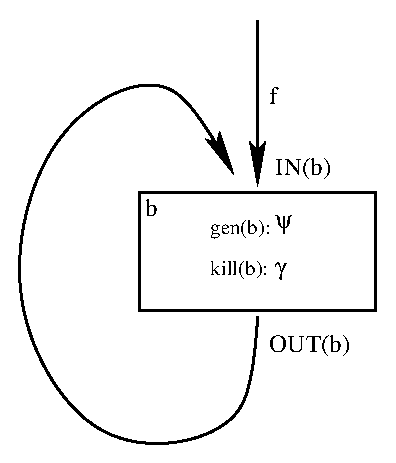
\includegraphics[scale=1]{Figure/figure_1} 
}
&
\scalebox{.7} {
\begin{tabular}{|c|c|c|}
\hline
Iteration & IN(b) & OUT(b) \\ \hline
\hline
$1$ & $f$									& $(f \wedge \KillSym) \vee \GenSym$ \\ \hline 
$2$ & $f \vee ((f \wedge \KillSym) \vee \GenSym)$	& 
			$\begin{array}{cl}
				& ((f \vee ((f \wedge \KillSym) \vee \GenSym)) \wedge \KillSym) \vee \GenSym \\
			 	=& (((f \vee (f \wedge \KillSym)) \vee \GenSym) \wedge \KillSym) \vee \GenSym \\
			 	=& ((f \vee \GenSym) \wedge \KillSym) \vee \GenSym \\
			 	=& (f \vee \GenSym \vee \GenSym) \wedge (\KillSym \vee \GenSym) \\
			 	=& (f \vee \GenSym) \wedge (\KillSym \vee \GenSym) \\
			 	=& (f \wedge \KillSym) \vee \GenSym \\
			\end{array}$ \\ \hline 
$3$ & $f \vee ((f \wedge \KillSym) \vee \GenSym)$	& $(f \wedge \KillSym) \vee \GenSym$ \\ \hline
\end{tabular}
}
\\ \\
 \footnotesize (a) Data Flow & \footnotesize (b) Data flow values per iteration \\
\end{tabular}
\label{fig:flowdiag}
\caption{The termination of computation of boolean functions}
\end{figure}


%%%%%%%%%%%%%%%%%%%%%%%%%%%%%%%%%%%%%%%%%%%%%%%%%%%%%
\section{Storage Requirement}
%%%%%%%%%%%%%%%%%%%%%%%%%%%%%%%%%%%%%%%%%%%%%%%%%%%%%

The memory requirement of our analysis consists of the
    storage space for the matrices ( $D_F$ and
    $I_F$ ) and the boolean functions.  Let $n \in
    \nat$ denotes the cardinality of the set $\heap$ at a
    program point. Obviously $n$ is bounded by the total
    number of pointer variables in the program. Let $m \in
    \nat$ denotes the maximum number of possible distinct
    pointer fields emanating from a heap directed pointer,
    which is again a bounded quantity. Between two pointer,
    for each field, we only use: (a) the ($k$-limited) count
    of the number of indirect paths starting at that given
    field, and (b) if there is a direct path using that
    field, the storage requirement for the matrices is
    bounded as:
\begin{eqnarray*}
\mbox{Space requirement for } D_F &:&  O(n^{2}* m) \\
\mbox{Space requirement for } I_F &:& O(n^{2} * m^2)
\end{eqnarray*}

The boolean functions at each program point are stored in an
expression tree.  As can be seen from the equations for the
boolean functions, the height and width of the expression
tree for a function is polynomial in the number of pointer
instructions in the program. By carefully reusing the trees
for the subexpressions in an expression, it is possible to
store the boolean functions efficiently.


%% \cmt{
%% \begin{figure}[t]
%% \centering
%% \begin{tabular}{@{}lc@{}}
%% {\small\tt
%%       \begin{tabular}[b]{l}
%%         S1. s$\rightarrow$f1 = p; \\
%%         S2. q$\rightarrow$f2 = s; 
%%       \end{tabular}
%%     } & 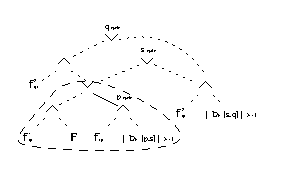
\includegraphics[scale=2]{Figure/figure_17} \\ 
%% \footnotesize
%% (a) A code fragment & 
%% \footnotesize (b) Expression tree storing the boolean
%% functions \\ 
%% & \footnotesize generated after {\tt S2}. \\
%%   \end{tabular}
%%   \caption{Scheme to store the boolean functions generated at
%%     each program point}
%% \label{fig:performance_storage}
%% \end{figure}
%% }
